The following chapter aims to explain the basic machine learning approaches used for this thesis.

\subsection{K nearest neighbor}
\label{cha:knn}
\acrfull*[]{knn} is a very simple classification algorithm for the numerical features used in this thesis.
First, the source dataset is converted into a vector representation. Each sample of the source dataset is represented as and $n$-dimensional vector, where $n$ is the amount
of features within that particular dataset. In addition to that vector the class of each sample is also saved.
The classification is achieved by representing a new sample within the aforementioned vector-space.
For the new sample the $k$ nearest neighbors are calculated using a distance metric, where $k$ is an odd-number. For this thesis the \textit{euclidean} distance was used.
The euclidean distance for two vectors($\mathrm{v}_{1},\mathrm{v}_{1}$) in the $n$ dimensional space is defined as follows:
\begin{equation*}
    euclidian(\mathrm{v}_{1},\mathrm{v}_{1}) = \sqrt[]{\sum_{i=1}^{n} (\mathrm{v}_{1,i} -\mathrm{v}_{2,i})^2} 
\end{equation*}
In the base version of \acrshort*[]{knn} the new sample is put in the same class as the majority of its $k$-neighbors.
In addition to that the $k$ nearest neighbors can also be weighted using their distance to the new sample\cite[]{Cunningham2022}. 

K nearest neighbor for this thesis has been implemented using the \href{https://scikit-learn.org/stable/index.html}{scikit-learn package}. 

\subsection{Random forest}
\label{cha:rf}
In the following the base concept of the random forest algorithm used for this thesis will be explained.
\\The random forest algorithm is a collection of identically distributed decision trees\cite[]{Breiman2001}.
The algorithm can be split into the creation of a bootstrapped dataset, the creation of decision trees and the evaluation of said trees.

\subsubsection*{Bootstrapping}
The goal of this step is to create a new dataset for each decision tree. This happens by randomly selecting 
samples from the source dataset. It is noteworthy that samples can be selected multiple times when creating such a bootstrapped dataset.
Furthermore, not all samples are included in each dataset. Those samples, which are not included in any dataset are called \textit{out-of-bag} samples 
and are later used for further tree enhancement. With those bootstrapped dataset decision trees can be built in the next step.

\subsubsection*{Creation of decision trees}
For each bootstrapped dataset a new decision tree is created using the following steps. Firstly a number of features is randomly selected.
For those selected features it is determined, which feature is best for splitting the data, so that the classes are separated very clearly.
This is usually determined using the \textit{Gini}-impurity.
The Gini-impurity is a measure of how well a dataset can be divided using a certain feature.

The Gini-impurity can be calculated at each node of a decision-tree and is ranged from 0 to 0.5.
Let $k$ be the number of classes and let $\mathrm{p}_{i}$ be the probability of a sample belonging to the class($i$) and the Gini-impurity($Gini(D)$) of the dataset($D$)
at a certain node within the tree can be defined as follows:
\begin{equation*}
    Gini(D) = 1 - \sum_{i=1}^{k} \mathrm{p}_{i}^2
\end{equation*} \cite[]{Karabiber}

After selecting the splitting feature the data is split and the whole process repeats for the newly created nodes.
When selecting a new splitting feature all features already existing in the tree can be used again. This whole process is 
repeated until every path of the tree leads to a clear classification result\cite[]{Breiman2001}.

\subsubsection*{Evaluation and optimization}
After the construction of the forest the performance can be evaluated using the out-of-bag samples.
This is achieved by classifying the samples from the out-of-bag dataset using the random-forest. Each tree within the forest is provided with the data from the sample
and votes for a class based on the samples features.

The parameters of a random forest, for example the number of features considered at each node, can be optimized. To achieve that multiple forests with 
different parameters are generated and the best performing one for the out-of-bag samples is selected\cite[]{Breiman2001}.

For this paper the random forest approach has been implemented using the \href{https://scikit-learn.org/stable/index.html}{scikit-learn package}. 


\subsection{Neural networks}
The idea to emulate neural system using computers was first discussed in the 1940s by McCulloch and Pitts\cite[]{McCulloch1943}. Since then the technology around neural networks has improved greatly. The following chapter describes the basic
concepts of \acrlong*[]{nn} and their implementation for this thesis.

The goal of neural networks in general is to process input data through an emulated brain-like structure for a multitude of machine learning tasks.
Neural networks are universally appliable algorithms due to their ability to resemble any given function through combining multiple smaller functions.
Furthermore, neural networks can be computed using matrix calculations, which are typically carried out on the graphics card of a system, as it is optimized for such operations\cite[]{Jain}.  
In this thesis neural networks are used to determine the activity of protein-ligand interactions using detailed interaction data.

\subsubsection*{Terminology}
A neural network consists of \textit{neurons} and \textit{synapses}. 
Neurons are nodes within the neural network that can take one or multiple inputs and transform them into one singular output.
The neurons are connected through synapses which can further manipulate values given to them by applying \textit{weights} and \textit{biases}\cite[]{Schmidhuber2015}.

A very simple neural network consists of an input neuron layer, where each neuron corresponds to a feature, a singular output neuron for binary classification. 
The neurons of the input layer are connected to the output neuron through synapses.

\subsubsection*{Classification using neural networks}
This section is dedicated to demonstrating the classification of a sample within already existing neural network with one hidden layer.
In a first step the features of the sample are mapped to the input neurons. After that the values are transferred to the hidden layer through the respective 
synapse. During this process the weight for that synapse is applied (this is usually done through a multiplication). Before the feature gets to the neuron of hidden layer 
the bias of that synapse is applied to the feature through an addition. Inside the neuron the value is modified using an activation function. Example for activation functions can be found 
in the \textit{activation functions} section within this chapter. All the modified values from the hidden layer are transported through synapses to the output neuron 
which calculates the class using an activation function\cite[]{Schmidhuber2015}.
\begin{figure}[H]
    \begin{center}
        \caption[]{neural network representation}
        \label{fig:nn_rep}
        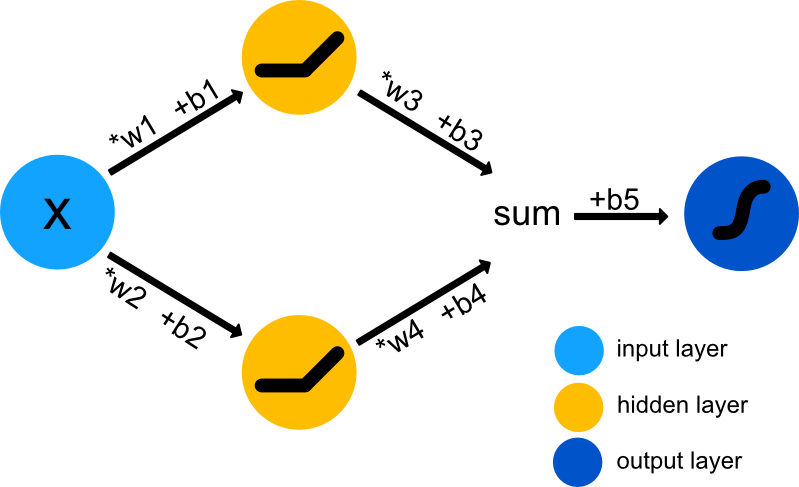
\includegraphics[width=9cm]{NN/feedforward.png}
    \end{center}
\end{figure}

\subsubsection*{Back propagation and gradient descent}
While the activation functions for the neural network can be set as parameters when creating the network the weights and biases are optimized during training.
To assess the performance of a set of weights and biases a loss function is used. The loss function determines how well the predicted values compare to the actual values\cite[]{Janocha2017}.
The \textit{\acrfull*[]{bce}} is an example for such a loss function and is defined for $n$ samples as follows:
\begin{equation*}
    BCE = \frac{1}{N}\sum_{i=1}^{N}target_i*log(predicted_i)+(1-target_i)*log(1-predicted_i)
\end{equation*}
\cite[]{Archdeacon1994}

With a loss function it is possible to optimize values using gradient descent. This is achieved by calculating the derivative of the loss function with respect to the parameter.
Initially the parameter will be initialized with a random value. After that the train set will be evaluated using this particular parameter. Then the derived loss function is applied to the values.
Using a fixed \textit{learning rate} the \textit{step size} for gradient descent is calculated by multiplying the learning rate with the result from the derivative loss function. 
For the next iteration of gradient descent the step size will be subtracted from the value to get a new optimization value.
Using this technique not every possible value of the variable needs to be examined. With a smaller proximity to the minimum the step size decreases \cite[]{Zhang2019}.
The following graph displays a loss function with the points demonstrating the variable values investigated by gradient descent.
\begin{figure}[H]
    \begin{center}
        \caption[]{gradient descent representation}
        \label{fig:gd_rep}
        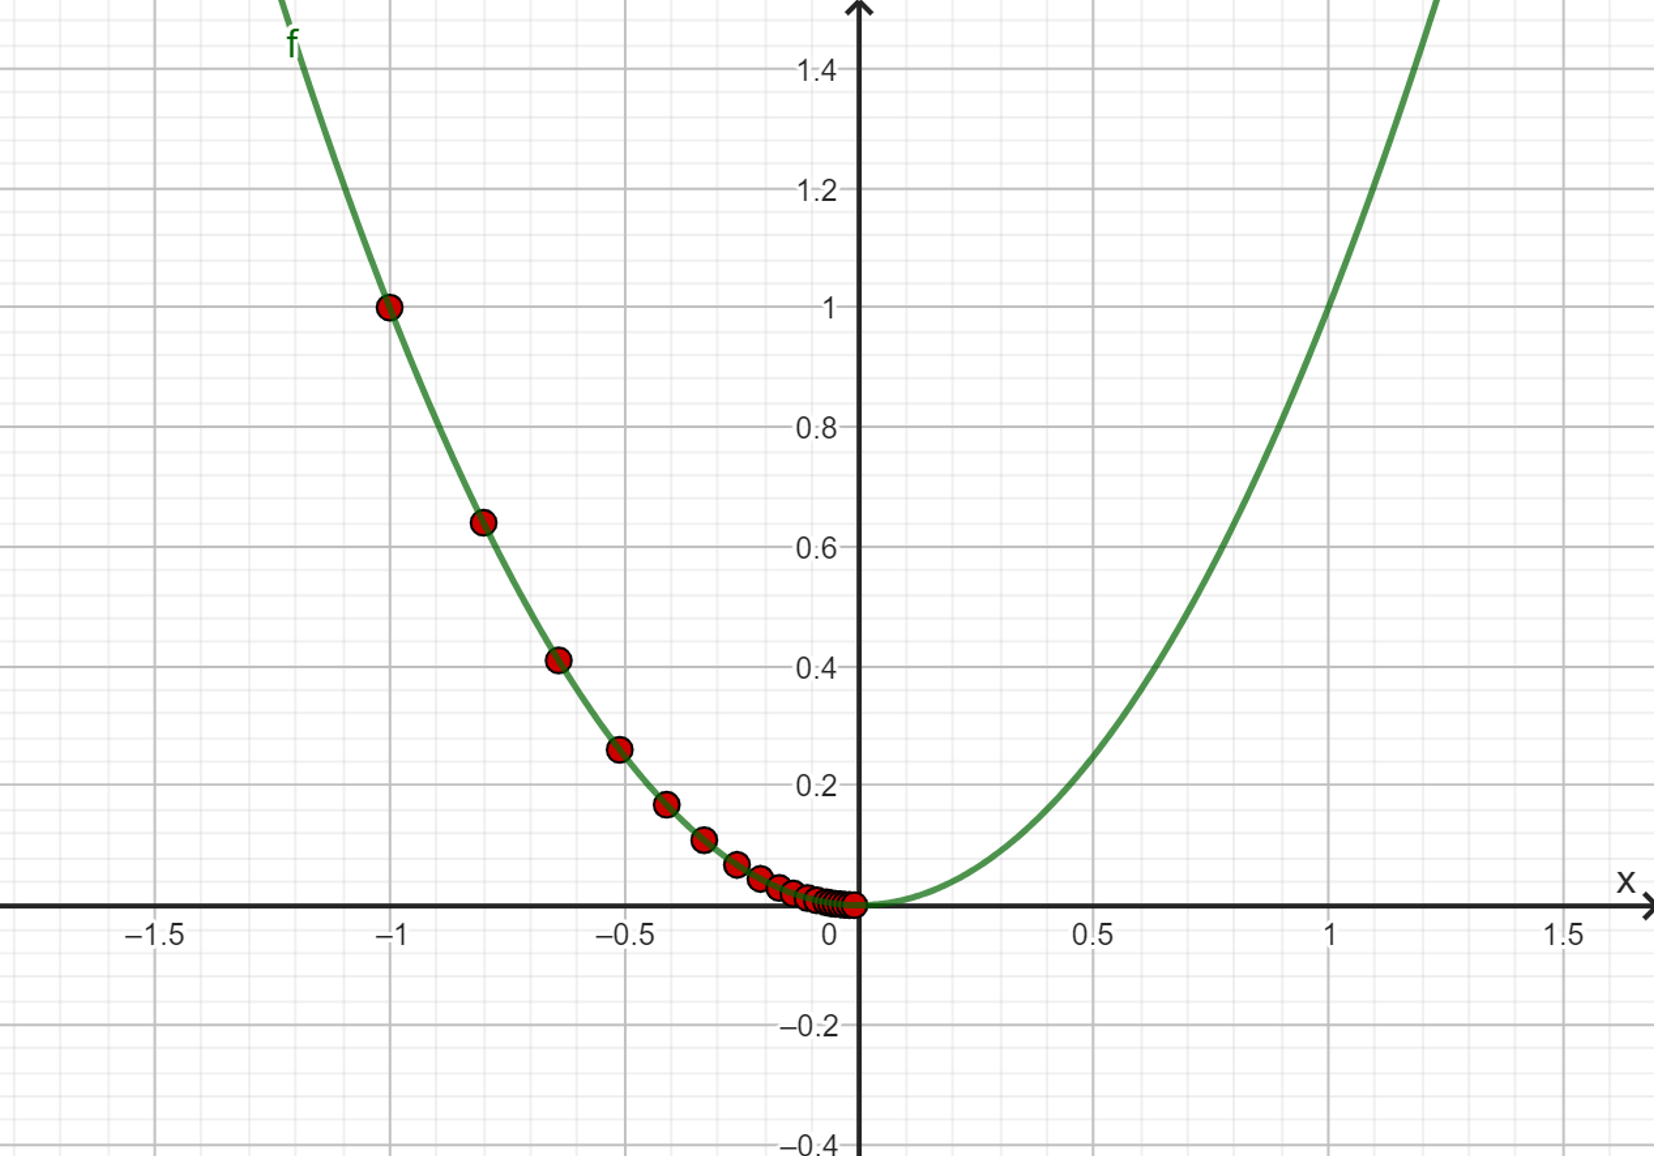
\includegraphics[width=9cm]{NN/gradient_descent.png}
    \end{center}
\end{figure}

Using this concept the \textit{back propagation} algorithm optimizes all the weights and biases within a neural network all at once.
The loss function is derived for each bias and weight. After that the resulting functions are applied to the values and new weights and biases are calculated using the step size.
This process is repeated until a certain threshold for the overall loss is reached or the number of iterations has reached its maximum\cite[]{Raschka2024}. 

\subsubsection*{Activation functions}
Activation functions play a major role in the performance of neural networks. They are specified when creating a new model. For this thesis the \textit{Sigmoid}
activation function was used for the output-layer. The sigmoid function is defined as follows:
\begin{equation*}
    \sigma(x) = \frac{e^x}{1+e^x}
\end{equation*}
\cite[]{InternationalWorkshoponArtificialNeuralNetworks1995Torremolinos1995}
The sigmoid function is very applicable for binary classification, as it provides values between 0 and 1 which can be interpreted as probabilities\cite[]{Zhang2021}.
The \textit{\acrfull*[]{relu}} activation function has been proven to improve performance when used in hidden layers\cite[]{Dubey2022}. Therefore, this function is used for the hidden layers within the neural network
implementation. \acrshort*[]{relu} is defined as follows:
\begin{equation}
    f(x)=max(0,x)
\end{equation}\cite[]{Dubey2022}

Different activation functions work for different datasets, it is therefore crucial to determine which activation function works best for the provided data. Other activation functions include
\textit{Tanh} or \textit{APL}\cite[]{Dubey2022}.

The practical neural network approach of this thesis has been implemented using the Tensorflow\cite[]{Abadi2016} library. The model definitions where optimized manually using the validation accuracy.
\label{cha:nn}



